\chapter{Multi-Agent Coordination, Information Routing, and Shared State}\label{ch:C21}
October 2026 LatComm replaces repeated text transfer with a reusable learned packet between frozen language models~\cite{lin2026latcomm}. It makes coordination a representation-compatibility problem as well as a scheduling problem: a receiver must interpret what another model encoded, under a finite communication budget. This is evidence from bounded question-answering experiments, not a demonstration that arbitrary autonomous teams share a sufficient state. The chapter therefore begins with task dependencies and proceeds to evidence contracts, latent channels, concurrent memory, and causal team evaluation.

Delegation changes the distribution of computation across contexts, models, tools, and execution times. It does not create additional evidence merely by creating additional agents. A team can improve coverage through parallel exploration, specialist interfaces, and independent checking, yet it can also multiply a shared misconception. The relevant research question is therefore conditional: which decomposition preserves the information required for the task, and when does the resulting gain exceed communication, coordination, and verification costs?

This chapter treats a team as a distributed decision system with explicit ownership and mutable state. The discussion separates parallel sampling from communication, role assignment from capability diversity, and workflow topology from actual execution semantics. AutoGen and MetaGPT provide influential examples of conversational and role-organized coordination~\cite{wu2023autogen,hong2023metagpt}. Their architectural patterns motivate comparisons; they do not license treating every multi-agent deployment as a stronger policy.

\section{Task graphs and the value of decomposition}\label{sec:C21:decomposition}
A task decomposition is a directed graph whose nodes represent work products and whose edges represent prerequisites. A node should specify a deliverable, evidence requirements, permitted tools, budget, and acceptance condition. ``Research the topic'' is too underspecified to support reliable integration. ``Identify contradictory primary results under the declared cutoff, returning source identity, claim, experimental population, and limitation'' defines an auditable information product. The distinction matters because integration quality depends on what the delegate was asked to preserve.

Let $G=(V,E)$ be an acyclic work graph, $w_v\geq0$ the execution time of node $v$, and $m\in\mathbb N_{>0}$ the worker limit. Ignoring communication and scheduling overhead, the makespan $T$ satisfies
\begin{equation}
 T\geq\max\left\{\frac{\sum_{v\in V}w_v}{m},
 \max_{p\in\mathcal P}\sum_{v\in p}w_v\right\},
\end{equation}
where $\mathcal P$ is the set of dependency paths. The first term is a work bound; the second is the critical-path bound. Adding workers cannot overcome a serial evidence dependency. Communication, verifier queues, tool contention, and failed retries increase observed makespan above this idealized lower bound.

The graph itself may be uncertain. A search task can reveal a missing prerequisite, invalidate a planned branch, or require another tool. Dynamic orchestration therefore operates over both task actions and graph-editing actions. A manager that repeatedly replans can spend more time maintaining the graph than the workers spend executing it. Graph-edit operations should have budgets and stopping rules, particularly when a model is rewarded for producing elaborate plans rather than verified progress.

Decomposition also changes statistical difficulty. Breaking a coherent task into subtasks may remove context that made the original problem solvable. Conversely, it can reduce distraction by exposing each worker to a narrower evidence set. A controlled experiment should distinguish these effects by comparing the same decomposition executed serially, in parallel without communication, and in parallel with communication. If only the communicating condition improves, evidence exchange is implicated. If serial decomposition already captures the gain, parallelism may primarily affect latency.

An important operating condition is interface stability. Delegation works best when a subtask produces a bounded artifact that can be checked independently of the worker's narrative. A parsed dataset, executable patch, or evidence table has a clearer acceptance surface than a general recommendation. This does not make artifact verification trivial, but it constrains where errors can enter integration. Tasks requiring continuous negotiation of a shared latent interpretation are harder to decompose safely than tasks with explicit data dependencies.

The graph also needs an invalidation relation. If node $v$ consumed artifact digest $d$ from node $u$, a later replacement of that artifact must mark $v$ and its affected descendants stale; graph reachability alone is insufficient when several artifact versions coexist. Reexecuting every descendant is conservative but potentially expensive. Reusing a descendant is justified only when its declared dependencies remain valid, or when an independently checked equivalence permits substitution. A model's statement that a revision is minor is not such an equivalence. This turns the critical path into a versioned evidence path: parallel work reduces elapsed computation only to the extent that its outputs survive integration without invalidating subsequent work. Chapter~\ref{ch:C32} applies the same dependency principle to deployed model, tool and memory updates.


\section{Independence diversity and correlated error}\label{sec:C21:dependence}
Independent samples and collaborating agents answer different questions. If each independent attempt succeeds with probability $p$, then the chance that at least one of $n$ attempts succeeds is $1-(1-p)^n$. This expression assumes independence and an oracle that identifies a valid attempt. A practical selector can reject the successful attempt or accept a plausible failure. Therefore the expression is headroom under a stated model, not an end-to-end reliability prediction.

For averaging, positive pairwise correlation inflates variance under a fixed marginal model. For $n\geq2$ Bernoulli outcomes $X_i\in\{0,1\}$ with common success probability $p\in(0,1)$, sample mean $\bar X=n^{-1}\sum_{i=1}^nX_i$, and feasible common pairwise correlation $\rho$, the variance of their mean is
\begin{equation}
 \operatorname{Var}(\bar X)=\frac{p(1-p)}{n}
 \left[1+(n-1)\rho\right].
\end{equation}
The expression follows by expanding the covariance sum; it does not require full joint independence. When $1+(n-1)\rho>0$, the variance-equivalent effective sample size is $n/[1+(n-1)\rho]$. A zero bracket is a degenerate zero-variance case for which that finite effective-size interpretation is undefined. It is only a variance equivalence, not a complete description of team success. Two joint distributions can share pairwise correlations while differing in the probability of all agents failing together.

Assigning different role names does not guarantee low correlation. Workers can share training data, model family, prompt assumptions, retrieval sources, and tool failures. A critic primed with the original answer may anchor on it even when told to be independent. A more meaningful diversity intervention varies information access, initial hypothesis, retrieval strategy, or verification method, then measures whether these changes reduce harmful dependence. Diversity that increases disagreement without improving error detection is not automatically useful.

Communication can destroy independence. Once workers see a popular hypothesis, later agreement may reflect copying rather than independent confirmation. An evidence protocol can preserve initial private assessments before discussion. Record each worker's claim, confidence interpretation, supporting observations, and falsification test; then permit exchange. Comparing pre-discussion and post-discussion judgments reveals whether communication corrects errors or amplifies consensus. The process remains an experiment rather than a proof that private reasoning is always preferable.

The causal baseline should spend the same total budget on a single agent, independent samples, and communicating teams. Equal call counts are insufficient when prompts, tool actions, and verifier work differ. Also report wall-clock under a declared concurrency limit. A team may reduce elapsed time while increasing total cost, which can be appropriate for time-critical work. The conclusion should state that tradeoff rather than describe parallelism as cost reduction.


\section{Messages as evidence-bearing interfaces}\label{sec:C21:messages}
A delegation message is an interface contract. Its payload should separate instructions, observations, inferences, proposed actions, and unresolved questions. Flattening them into one natural-language paragraph forces the receiving model to reconstruct authority and provenance. This is especially dangerous when a worker quotes untrusted material that contains instructions. The manager must not treat quoted source content as a delegated command merely because it arrived through an internal agent channel.

An evidence-bearing result contains a claim identifier, source references, the relevant observation, the transformation applied, uncertainty, and applicability conditions. For a code change it includes the artifact digest, tested revision, test selection, and known failures. For a research claim it includes paper version, result location, population, baseline, and limitation. The representation can be structured JSON or another schema; the important property is that integration can validate required fields and inspect the source behind them.

Schema validity does not establish semantic validity. A worker can provide a well-formed citation that does not support the associated claim. Therefore validation must be layered. Structural validation checks field presence and types. Referential validation resolves identifiers and versions. Evidential validation tests whether the cited observation supports the inference. Task validation checks whether the work product addresses the delegated objective. Conflating these stages makes a successful parser appear to be a scientific verifier.

Compression at handoff introduces an information bottleneck. Suppose a worker observes $O$, emits message $Z$, and the manager chooses an action from $Z$. If two possible observations require disjoint correct actions but induce the same $Z$ and the same other manager information, no rule on that information can be correct on both. Prior knowledge or a follow-up observation can change the information set; the claim is not that all omitted text is unrecoverable. The data-processing principle motivates preserving sufficient evidence rather than only conclusions. In practice exact sufficient statistics are unknown, so interfaces should expose provenance links and permit targeted follow-up retrieval.

A useful failure case is a worker reporting that ``the benchmark improved'' while omitting that the improvement used additional attempts or a different evaluator. The manager integrates the result as a method gain, and the final synthesis becomes incorrect even though neither agent invented a number. A required comparison field would have exposed the mismatch. This example illustrates why evidence loss at handoff is a distinct error class from hallucination and deserves separate measurement.

Message cost also affects scaling. For a round in which each of $n$ workers emits an $L$-bit message to every other worker, payload volume is $n(n-1)L$ before protocol overhead. A star that sends those reports once to a manager and broadcasts an $L_b$-bit summary uses $nL+nL_b$ bits, but holding $L_b$ fixed can discard task-relevant distinctions. The bound is an accounting model, not a measured speedup or a guarantee that the summary is sufficient. Hierarchical summaries reduce volume but introduce another compression layer and a potential single point of epistemic failure. Topic-based routing and shared artifact stores can reduce duplication, provided access control and version identity remain explicit. The appropriate topology depends on the dependency graph; a universal full-mesh conversation is rarely a neutral baseline.

\subsection{Learned latent channels and representation compatibility}\label{sec:C21:latent}
Text is only one communication substrate. LatComm's October 2026 preprint encodes a context once, without a question, into fixed-size hidden-state slots; a different frozen receiver reads them through learned cross-attention and prompt-dependent gates. Its two stages train the interface, then freeze the compressor while adapting reader-interface and gate parameters for question answering; both LLM backbones remain frozen~\cite{lin2026latcomm}. Interlat instead studies direct last-layer-state communication and learned compression, including heterogeneous sender--receiver configurations~\cite{du2026interlat}. These mechanisms require access below a typical text-only hosted API. They must not be inferred from ordinary agent handoff support.

To compare such systems, let $x\in\mathcal X$ be sender evidence, $q\in\mathcal Q$ a receiver request, and $y\in\mathcal Y$ the target. A general channel has an encoder $e_\phi:\mathcal X\rightarrow\mathbb R^{p\times s\times d}$, a transport or quantization map $Q_b$, and a receiver distribution $p_\psi(y\mid q,z)$ with $z=Q_b(e_\phi(x))$. Here $p,s,d\in\mathbb N_{>0}$ are channel-group count, slots per group and slot width (with $p=1$ for a single group), and $b\in\mathbb N_{>0}$ is the stored bits per scalar. Under a fixed task distribution and nonnegative predictive-distribution loss $\ell$ (such as log loss), one possible joint design objective is
\begin{equation}
 \min_{\phi,\psi}\;
 \mathbb E\!\left[\ell\{p_\psi(\cdot\mid q,z),y\}
 +\lambda_B B(z)+\lambda_T T(x,q,z)\right].
\end{equation}
The weights $\lambda_B,\lambda_T\geq0$ convert transmitted bits $B$ and end-to-end time $T$ to the chosen objective units. This is a comparison formulation, not the objective attributed to either paper. Frozen-backbone methods restrict the trainable parameters to adapters, compressors, or readers. A reconstruction objective and a task objective impose different information preferences; successful reconstruction is not sufficient for correct action, while task-only optimization can discard distinctions needed by future requests outside the training distribution.

The channel's nominal payload is $psdb$ bits before headers and error-control overhead, but token count is an inadequate measure of its cost. The sender may process every evidence token, the receiver attends to slots at selected layers, and each sequential agent can retain a growing cache. Count transmitted tensors, storage copies, dtype conversions, encoder FLOPs, additional receiver attention, and device transfers. A comparison that charges generated text tokens to a text team while excluding latent tensors and extra hidden-state computation gives the methods different accounting boundaries. Conversely, text may be repeatedly tokenized and prefetched when a packet is reusable; reuse count and cache policy must therefore be matched.

Compatibility is semantic as well as dimensional. A width-matching projection does not establish that a new receiver assigns the same meaning to an old packet. Replacing the sender checkpoint, changing selected layers, quantizing the packet, or retraining the decoder changes the channel. Record an encoder--packet--reader compatibility identity and test migration with frozen packets as well as regenerated packets. If only regenerated packets work, the system has demonstrated a new channel, not backward-compatible memory. A context packet also needs source identity, validity interval, permissions, and deletion dependencies outside its latent values; a dense vector cannot be assumed to carry an enforceable authority label.

The inspected LatComm implementation makes this boundary identifiable: \texttt{LatentBridge.compress} constructs the packet, \path{LatCommModel.encode_context} obtains its encoder input, \texttt{LatentInjector} inserts receiver-side transformations, and \texttt{PacketCache} manages stored packets~\cite{lin2026latcomm}. These callable definitions were read at a dated source revision; they were not executed here. Their existence establishes an implementation path, not numerical parity with the paper or robust compatibility after modification.

The packet shape and cache key matter in the released code. \path{LatentBridge.compress} returns one slot array per paired layer, so a context packet is $[p,s,d]$, not merely $[s,d]$. \texttt{PacketCache} selects that packet by a hash of context text and loads its stored dtype; this lookup does not itself validate an encoder--reader compatibility identity. The generation path computes prompt-conditioned gates and reuses them during decoding~\cite{cumb2026latcommcode}. These observations bound the implementation claim: a wrapper must bind cache namespace and packet generation to the selected checkpoints and layer pairs. A matching text hash, shape or dtype alone does not establish semantic compatibility, and storage at 16 bits does not imply every consumer-side copy remains 16-bit. No mismatched-cache benchmark outcome is asserted.

A discriminating experiment compares raw text, equal-byte text compression, a single-vector representation, and a multi-slot channel under the same sender evidence, receiver, task stream, and total compute envelope. Include unseen questions about a fixed document and new document types; a query-independent packet should be tested on questions unavailable when it was encoded. Swap in mismatched packets as a negative control, remove the channel, and vary packet precision. Measure action correctness, contradiction handling, calibration, and effect-policy compliance alongside bandwidth and latency distributions. For model migration, cross old and new encoder--reader pairs and retain the off-diagonal failures. A large speed gain on repeated multiple-choice reading would remain useful, but would not by itself establish reliable sharing of open-ended plans, revocable authority, or concurrent agent state.


\section{Shared memory and conflicting writes}\label{sec:C21:sharedmemory}
Shared memory is a distributed database whose contents influence policy. Consequently, concurrency errors can become reasoning errors. Two agents may update a fact from different observations, overwrite each other's progress, or retrieve an obsolete skill after another worker changes its assumptions. The required consistency level depends on the record's semantics. Append-only evidence can often tolerate concurrent insertion; a current authorization grant cannot be resolved by choosing whichever natural-language summary sounds more persuasive.

Separate immutable observations from mutable interpretations. Observations carry source, time, object version, and principal. Interpretations cite the observations they depend on and declare a validity interval. A correction can then invalidate an interpretation without destroying the evidence explaining why it was previously adopted. This structure supports both auditing and policy migration. It also prevents a deduplication routine from merging contradictory evidence into a falsely certain consensus.

Optimistic concurrency control is useful when updates are infrequent relative to reads. A worker reads version $v$, computes a candidate update, and commits only if the stored version remains $v$. On conflict it must re-evaluate the update against current state. Automatically replaying the old text can reintroduce a revoked fact. The conflict handler is therefore part of the policy interface, not simply a database retry loop.

Different merge functions have different algebraic properties. Set union is associative and commutative for immutable evidence identifiers. Last-writer-wins is operationally simple but uses clock order as a surrogate for semantic authority. Confidence-weighted merging can be misleading when confidence estimates share a common source or when the older record is more authoritative. A memory service should expose the selected rule and its assumptions rather than claim that all conflicts are solved by embeddings.

Procedural memory adds compatibility constraints. HyperSkill organizes skills and subtasks through trajectory hyperedges and maintenance operations~\cite{xu2026hyperskill}. This offers a concrete mechanism for relational reuse, but a shared deployment must additionally define whether two workers may prune or merge the same skill concurrently. The paper's sequential evaluation does not establish those concurrency semantics. A production adaptation should isolate maintenance, version skill identities, and preserve references from trajectories whose interpretation would otherwise change.

Evaluation should inject conflicting writes with known authority order, not merely test that both records appear in storage. Measure lost updates, stale reads that change decisions, unauthorized cross-user retrieval, and reproducibility of replay. Include a simple isolated-memory baseline: sharing is beneficial only when the transferred information improves the receiving task enough to justify contention, contamination, and governance complexity.


\section{Ownership cancellation and failure propagation}\label{sec:C21:ownership}
Every delegated operation needs an owner responsible for its budget, authority, cancellation, and final integration. A manager that starts workers and then terminates can leave active processes with no accountable controller. Ownership should be represented in execution state, with child operations linked to parent task and policy epochs. A child cannot acquire permissions merely because its parent was authorized to delegate reasoning.

Delegation authority is narrower than tool authority. A worker may be allowed to inspect a repository but not publish a branch, or to retrieve enterprise documents but not export them. Passing an unrestricted service credential to every worker defeats role isolation. Capability-scoped credentials and application-enforced tool registries make the distinction executable. The language model's stated role is useful task guidance, but it is not an access-control boundary.

Cancellation has two meanings: stop producing additional work and stop all ongoing effects. The former may be achievable immediately; the latter can require tool-specific termination or reconciliation. If one worker completes the task, cancelling redundant workers should not discard evidence of requests already dispatched. The system needs an outstanding-operation set and a rule for handling late responses. Otherwise a result can arrive after the manager has finalized and silently mutate shared memory.

Failure propagation should distinguish dependent and independent branches. If a shared prerequisite is invalidated, every descendant that used it may require reevaluation. An unrelated worker can continue. This can be implemented with artifact dependency digests rather than broad restart signals. A global restart is simpler but increases cost and can repeat external effects. Overly narrow invalidation is cheaper but risks integrating work derived from obsolete premises.

The tail behavior of a team often depends on stragglers. Waiting for every worker maximizes coverage but can make latency dominated by one failed dependency. Quorum completion can reduce latency but changes the evidence population and may systematically omit difficult or dissenting analyses. The stopping rule should specify whether missing workers count as failures, censored observations, or intentionally unused candidates. A post hoc choice of whichever stopping rule makes the run look best is evaluation leakage.

Fault-injection tests should combine worker loss, delayed messages, policy revocation, and shared-store outages. Independent single faults are easier to diagnose, but correlated failures are operationally important: one tool outage can affect all workers, while one poisoned shared memory can redirect the whole team. Report containment and benign completion together. A coordinator that avoids every incident by refusing delegation has not demonstrated useful orchestration.


\section{Experiments that isolate coordination mechanisms}\label{sec:C21:experiments}
A factorial design can vary decomposition, communication, model diversity, and memory sharing. The basic conditions are a single agent, serial specialists, parallel independent specialists, and communicating specialists. Each uses the same task set, tool fixtures, evaluator access, and resource accounting. The design should declare whether it matches money, tokens, elapsed time, or more than one envelope. Different matches answer different questions; they should not be mixed into one headline ranking.

For a fixed task instance $i$, define the paired gain $\Delta_i=Y_i^{\mathrm{team}}-Y_i^{\mathrm{base}}$. Average gains should be accompanied by their distribution over task families and difficulty strata. A positive mean can hide large regressions in tasks requiring coherent global context. Repeated model samples are nested within task instances, and shared persistent memory can induce dependence across tasks. Resampling individual calls as if they were independent produces overly narrow uncertainty intervals.

Communication ablations should preserve available information when possible. Removing all messages can change both coordination and evidence access. A stronger control supplies the same evidence through a deterministic aggregator while removing agent discussion. Conversely, randomizing or delaying selected messages tests whether timing and ordering drive the result. Such interventions can distinguish helpful information exchange from social anchoring or redundant narration.

Verifier access must be matched. A team with a dedicated critic effectively has more inference and perhaps additional tools. Compare it with a single agent receiving the same executable feedback, and with independent candidates selected by the same critic. If the gain comes from the critic rather than collaboration, the result still matters, but the mechanism should be named accurately. A critic's agreement is not oracle truth; its false acceptance and false rejection require independent audit.

The main failure taxonomy separates decomposition errors, worker errors, communication loss, shared-state conflict, integration errors, and verifier errors. A final wrong answer may involve several stages. Assigning all failures to the last agent obscures causal structure. Use seeded faults and counterfactual replay to test whether replacing a particular message or artifact changes the outcome. Replay is informative only when external state and model nondeterminism are controlled or explicitly accounted for.

These experiments are a proposed research program rather than results established by the cited frameworks. Their practical value is to make a claim such as ``multi-agent reasoning helps'' operational. The claim becomes a statement about a particular topology, information protocol, task distribution, and budget. That precision allows disagreement between studies to be investigated rather than averaged away.

The October 2026 coding-team study directly varies which workflow stage receives workers: planning, implementation or verification~\cite{samway2026codingteams}. In its ProgramBench configurations, planning delegation captures a different reward--cost tradeoff from adding implementers or verifiers; inexpensive workers are not interchangeable across roles. This is a configured empirical result, not a general law that planning is always the best allocation. The study does not evaluate team safety. Its mechanism suggests a sharper ablation than team size alone: preserve the lead, budget and information access, vary the recipient stage, and measure integration work as well as worker output. A cheap planner can supply a useful alternative hypothesis while a cheap implementer creates edits the lead must repair. The relevant causal mediator is useful accepted work after integration, not the number of delegates or messages. Testing that mediator requires recording rejected plans, conflicting patches and redundant verification so hidden consolidation cost cannot be mistaken for free parallelism.


\section{A bounded integration protocol}\label{sec:C21:integration}
The integration step should be designed as carefully as worker execution. A manager receives candidate artifacts, validates their provenance, identifies disagreements, and chooses whether more work is justified. It should not simply concatenate worker summaries and ask another model to produce a fluent answer. Concatenation preserves text but does not resolve incompatible assumptions, duplicated evidence, or different interpretations of the task.

One useful protocol maintains a claim graph. Nodes are claims or artifact predicates; edges identify supporting evidence, contradiction, or dependency. Workers submit proposed graph updates rather than final conclusions alone. The manager checks whether two claims concern the same population, version, and resource envelope before labeling them contradictory. Apparent disagreement can disappear when one worker reports author results and another reports an independent reproduction under a different environment. Genuine unresolved disagreement should remain visible.

Integration can stop when all required predicates have accepted evidence, unresolved contradictions have been represented, and the remaining expected value of additional work is below its cost under the declared objective. This stopping rule is conceptual because value estimates are uncertain. An implementation can approximate it with bounded rounds, explicit missing-evidence categories, and a limit on repeated requests for the same information. The approximation should be evaluated rather than presented as optimal metareasoning.

The protocol also needs a quarantine path. A worker result containing unverifiable citations, unexplained external changes, or suspicious instructions should be retained for diagnosis without entering trusted shared memory. Quarantine is not deletion and does not itself prove maliciousness. It prevents uncertainty about one artifact from silently becoming authority for subsequent actions. False quarantines reduce useful throughput, so their rate belongs in the evaluation alongside successful containment.

For a scientific review task, integration should retain disagreements over contamination, baseline strength, and statistical uncertainty even when the final narrative would be simpler without them. For a coding task, it should retain a failing regression test rather than allow a worker's confident explanation to supersede it. For enterprise actions, it should recheck authorization at the effect boundary. These examples share a principle: evidence and authority are properties of records and current policy, not consequences of a worker's role label.

The resulting team is best understood as a controlled distribution of computation and evidence. Parallelism supplies opportunities for coverage and latency reduction. Typed handoffs preserve what each opportunity discovered. Shared-state protocols prevent those discoveries from becoming incoherent or unauthorized. Independent evaluation determines whether the arrangement improves useful outcomes. None of these layers can be omitted by appealing to the number of agents or the apparent sophistication of their conversation.

\section{When isolation is the stronger coordination mechanism}\label{sec:C21:isolation}
Consider two workers preparing changes to different modules of one repository. Their edits appear independent, but both modify a shared interface specification. A shared writable checkout permits immediate coordination through the filesystem, yet it also permits one worker to test a transient mixture of changes. The resulting passing test verdict may correspond to no committed artifact. A later merge can then fail despite both workers reporting success. This is an evidence-identity failure rather than a lack of programming ability.

An isolated-workspace design gives each worker a base revision and a separate branch. The manager merges their artifacts and runs integration checks on the merged digest. This adds storage and validation cost but creates a clear causal boundary: worker tests concern branch artifacts; integration tests concern the combined artifact. If the interface changes are incompatible, the conflict is explicit. Isolation does not prevent semantic incompatibility, but it prevents accidental shared state from concealing it.

The same reasoning applies to research. Two investigators can independently inspect conflicting papers before receiving each other's conclusions. Their private notes preserve the evidence that motivated each interpretation. Discussion then operates on the disagreement rather than on an already homogenized summary. Complete isolation would prevent useful correction, so the design uses staged disclosure: independent extraction first, evidence exchange second, joint interpretation third. The stages allow an experiment to observe where agreement arises.

For memory systems, isolation can be temporary and selective. A worker may read a shared evidence snapshot while writing candidate interpretations to a private namespace. A promotion gate checks provenance, conflicts, and applicability before moving those interpretations into shared memory. This resembles a database transaction but adds semantic evaluation. The gate can still make mistakes, and its acceptance threshold determines the tradeoff between contamination and delayed learning. Promotion should therefore retain the original candidate and gate verdict for later audit.

The cost of this mechanism grows with candidate volume. If every worker proposes many redundant records, verification can dominate execution. Deduplication before promotion reduces load, but semantic deduplication can incorrectly merge distinct conditions. A safer first stage deduplicates exact source identities and artifact hashes; a later stage considers whether two interpretations are equivalent under their stated scope. Keeping these stages separate makes it possible to attribute errors to retrieval, deduplication, or review.

An evaluation should compare immediate shared writes, snapshot reads with private writes, and fully isolated memory under the same task sequence. Inject one incorrect but plausible record and measure its propagation, subsequent correction, and effect on task outcomes. Also include a valid rare record: a system that blocks all unusual memories may contain contamination while preventing beneficial transfer. Measure both harmful propagation and useful adoption, along with the review work needed to distinguish them.

The implication is conditional rather than categorical. Shared state is valuable when its information benefits exceed its coordination and contamination costs. Isolation is valuable when it preserves evidence identity, authority boundaries, or independent judgment. A principal design decision is to choose the smallest shared surface required for the task. Increasing communication and memory visibility without identifying the dependency they serve is not a scientific explanation of why a team should improve.


Figure~\ref{fig:C21:overview} isolates the mechanism and its stated information boundaries.
\begin{figure}[!htbp]
\centering
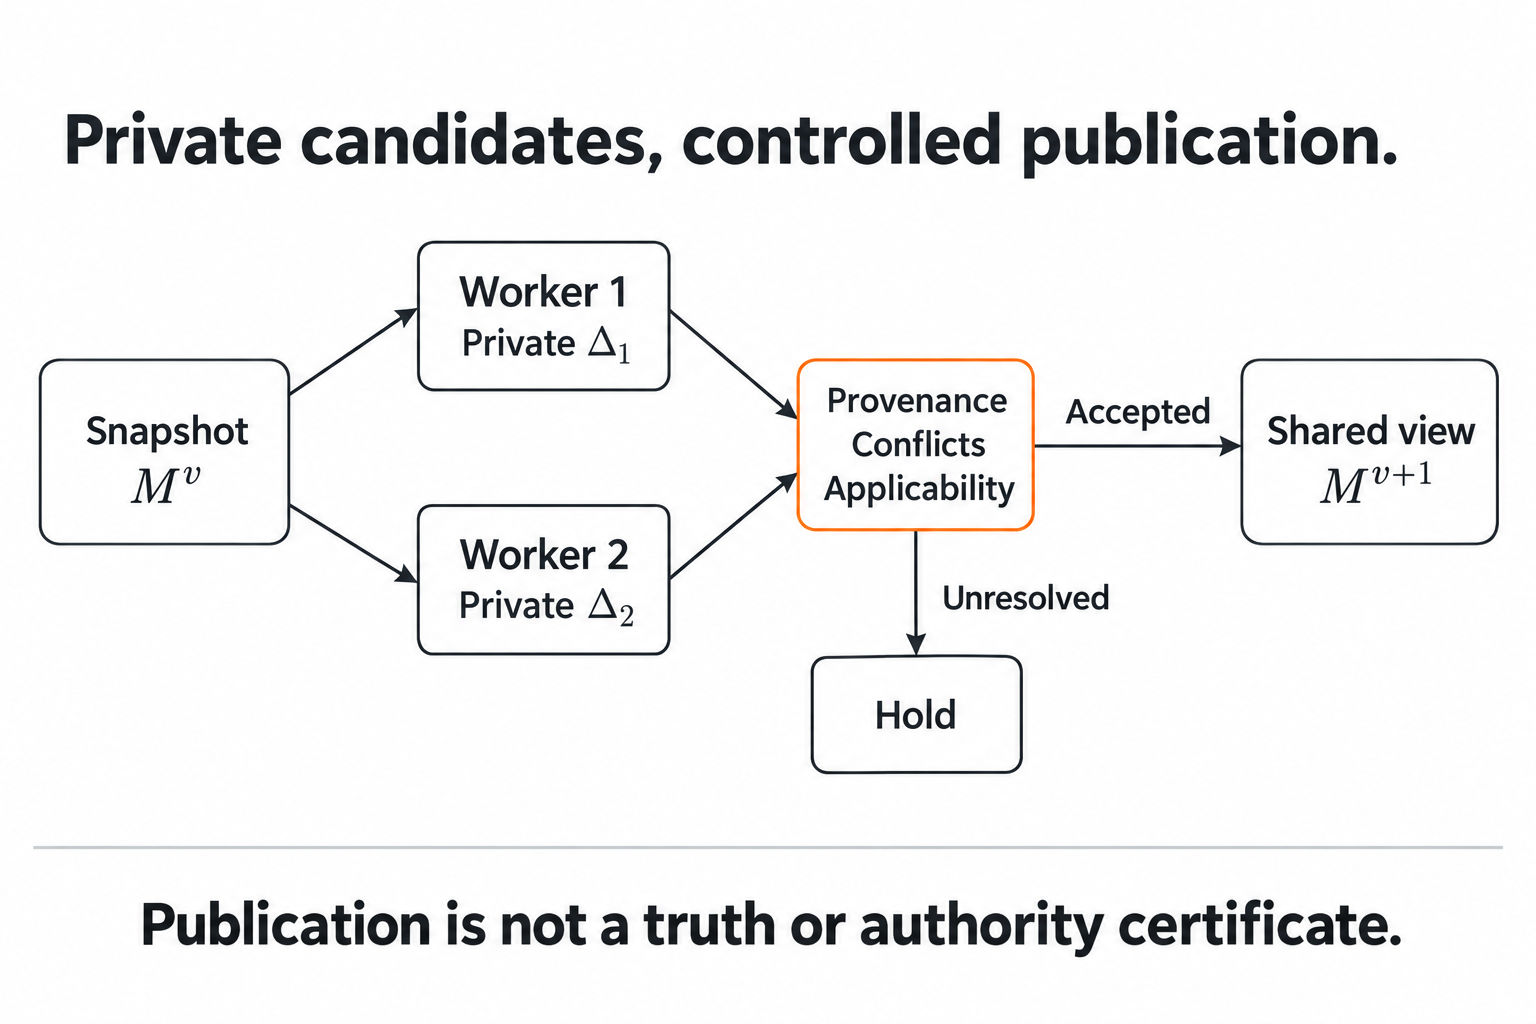
\includegraphics[width=\linewidth]{book/figures/assets/F21review.png}
\caption{Workers can read one versioned snapshot while retaining candidate interpretations privately. Only the promotion path publishes accepted candidates into a new shared view; unresolved candidates remain separate. Provenance, conflict and applicability checks retain an auditable decision boundary. The gate does not establish semantic truth, current effect authority, or a performance improvement.}
\label{fig:C21:overview}
\end{figure}

